\section{Ereignis und Wahrscheinlichkeit}

\subsection{Experimente und Ereignisse}

\begin{minipage}{0.35\columnwidth}
	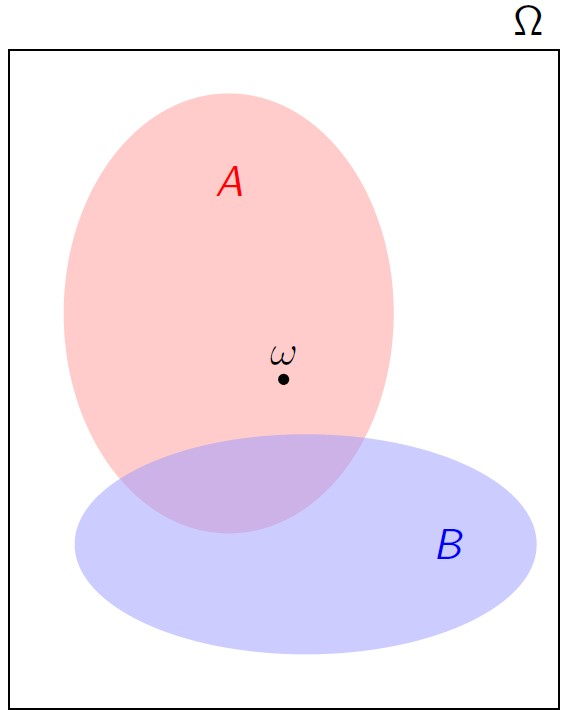
\includegraphics[width=\columnwidth]{images/ereignisse_begriffe.jpg}
\end{minipage}
\hfill
\begin{minipage}{0.55\columnwidth}
	\myul{\textbf{Elementarereignis $\bm{\omega}$}} \\
	Ausgang eines Experiments

	\vspace{0.2cm}

	\myul{\textbf{Experimente $\bm{\Omega}$}} \\
	Menge der möglichen Elementarereignisse $\omega$ 

	\vspace{0.2cm}

	\myul{\textbf{Ereignis}} \\
	Teilmenge von $\Omega$ \\
	\crd{$A$} eingetreten \textlrarrow\ Versuchsausgang $\omega \in \crd{A}$ \\
	\cbl{$B$} nicht eingetr. \textlrarrow\ Versuchsausgang $\omega \notin \cbl{B}$ 
\end{minipage}


\subsection{Spezielle Ereignisse}

\subsubsection{Sicheres Ereignis}

Das Ereignis $A = \Omega$ tritt immer ein: $ A = \Omega \subset \Omega $


\subsubsection{Unmögliches Ereignis}

Das Ereignis $B = \emptyset$ tritt nie ein: $ B = \emptyset = \{ \} \subset \Omega $


\subsection{Ereignis-Algebra}

\renewcommand{\arraystretch}{1.4}
\begin{tabular}{|l | l | l |}
	\hline
				& $A \cup B$ 												& $A$ oder $B$ 							\\
	Ereignisse 	& $A \setminus B$ 											& $A$, aber nicht $B$ 					\\
				& $\Omega$ 													& Alles (Sicheres Ereignis) 			\\
	\hline
 				& $\emptyset = \Omega \setminus \Omega$ 					& Alles ohne alles (Unmögl. Ereignis) 	\\

	Folderungen & $\overline{A} = \Omega \setminus A$ 						& Alles ohne $A$						\\

				& $A \cup B = \overline{\overline{A} \cap \overline{B}}$ 	& De Morgan 							\\
	\hline
\end{tabular}
\renewcommand{\arraystretch}{1}


\subsubsection{Rechenregeln}

\begin{minipage}[t]{0.48\columnwidth}
	\renewcommand{\arraystretch}{1.2}
	\begin{tabular}{l}
		$A \cap (B \cup C) = ( A \cap B) \cup ( A \cap C )$ 	\\
		$A \cup (B \cap C) = (A \cup B) \cap ( A \cup C )$ 
	\end{tabular}
	\renewcommand{\arraystretch}{1}
\end{minipage}
\hfill
\begin{minipage}[t]{0.48\columnwidth}
	\renewcommand{\arraystretch}{1.2}
	\begin{tabular}{l}
		$\overline{A \cap B} = \overline{A} \cup \overline{B}$ \\
		$\overline{A \cup B} = \overline{A} \cap \overline{B}$ 
	\end{tabular}
	\renewcommand{\arraystretch}{1}
\end{minipage}


\subsection{Wahrscheinlichkeit}

Definition der Wahrscheinlichkeit:
$$ \boxed{ P(A) = \lim\limits_{\text{\# Versuche} \to \infty} \frac{\text{\# Versuche, bei denen $A$ eintritt}}{\text{\# Versuche}} } $$


\subsubsection{Axiome}

\begin{itemize}
	\item Wertebereich: $0 \leq P(A) \leq 1$ 
	\item Sicheres Ereignis: $P(\Omega) = 1$ 
	\item Disjunkte Vereinigung (keine Schnittmengen zwischen Ereignissen)\\
	$P(A_1) \cup P(A_2) \cup ... \cup P(A_n) =  P(A_1) + P(A_2) + ... + P(A_n)$ 
\end{itemize}


\subsubsection{Eigenschaften}

\begin{itemize}
	\item Unmögliches Ereignis: $P(\emptyset) = 0$ 
	\item Komplementärereignis: $P(\overline{A}) = 1 - P(A)$
	\item Differenz: $P(A \setminus B) = P(A) - P(A \cap B)$
	\item Vereinigung: $P(A \cup B) = P(A) + P(B) - P(A \cap B)$
\end{itemize}


\subsection{Spezielle Arten von Experimenten}

\subsubsection{Laplace-Experimente}

Alle Versuchsausgänge haben die \textbf{gleiche Wahrscheinlichkeit} 
$$ \boxed{ P(A) = \frac{\text{Anzahl günstige Ausgänge}}{\text{Anzahl mögliche Ausgänge}} = \frac{\vert A \vert}{\vert \Omega \vert} }$$

Beispiele: (faire) Würfel, Karten ziehen, (faire) Münzen werfen


\subsubsection{Bernoulli-Experimente}

Genau \textbf{zwei }Versuchsausgänge mit Wahrscheinlichkeiten $p$ und $1-p$
$$ \boxed{ p = P(A), \qquad 1 - p = 1 - P(A) = P(\overline{A}) } $$


\subsection{Bedingte Wahrscheinlichkeit}

Die Bedingte Wahrscheinlichkeit ist die Wahrscheinlichkeit für \crd{$A$}, wenn \cbl{$B$} bereits eingetreten ist: 

\begin{minipage}{0.48\columnwidth}
	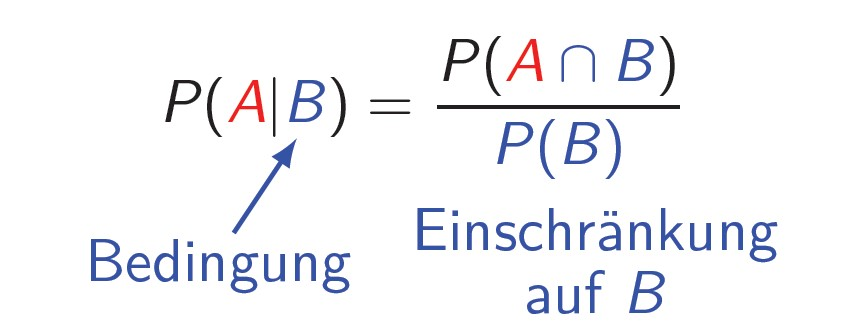
\includegraphics[width=\columnwidth]{images/bedingte_wahrscheinlichkeit.jpg}
\end{minipage}
\hfill
\begin{minipage}{0.48\columnwidth}
	\textbf{Im Allgemeinen ist}
	$$P(A|B) \neq P(B|A)$$
\end{minipage}


\subsubsection{Unabhängigkeit}

$A$ und $B$ heissen \textbf{unabhängig}, wenn
$$ \boxed{ P(A \cap B) = P(A) \cdot P(B) } $$

\vspace{0.2cm}

\begin{minipage}[t]{0.48\columnwidth}
	\begin{center}
		\myul{\textbf{Unabhängig}}

		\vspace{-0.5cm}

		$$ P(A|B) = P(A| \overline{B}) $$
		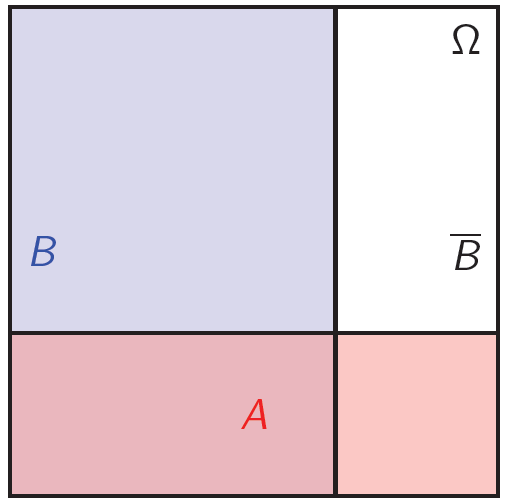
\includegraphics[width=0.6\columnwidth, align=t]{images/unabhaengig.png}
	\end{center}
\end{minipage}
\hfill
\begin{minipage}[t]{0.48\columnwidth}
	\begin{center}
		\myul{\textbf{Abhängig}}

		\vspace{-0.5cm}

		$$ P(A|B) < P(A| \overline{B}) $$
		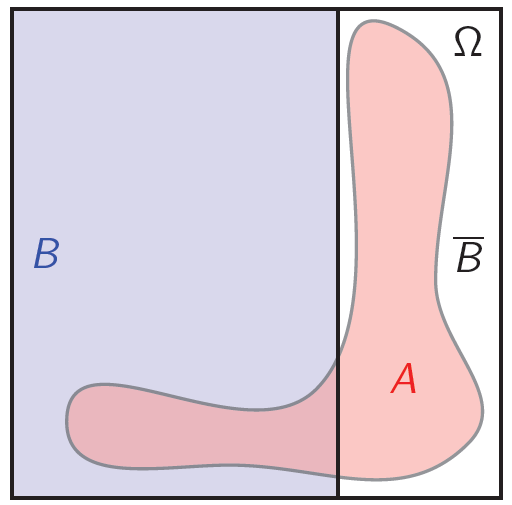
\includegraphics[width=0.6\columnwidth, align=t]{images/abhaengig.png}
	\end{center}
\end{minipage}


\subsection{Satz von Bayes}

Es gibt einen Zusammenhang zwischen den Wahrscheinlichkeiten, je nachdem welches Ereignis zuerst eintreten muss

$$ P(A \, | \, B) \cdot P(B) = P(A \cap B) = P(B \, | \, A) \cdot P(A) $$
\vspace{0.2cm}

\begin{minipage}{0.48\columnwidth}
	$$ \boxed{ P(A \, | \, B) = P(B \,| \, A) \frac{P(A)}{P(B)} } $$
\end{minipage}
\hfill
\begin{minipage}{0.48\columnwidth}
	$$ \boxed{ P(B \, | \, A) = P(A \,| \, B) \frac{P(B)}{P(A)} } $$ 
\end{minipage}

\vspace{0.2cm}
$$ \text{Wichtig: } P(A \, | \, B) = 1 - P( \overline{A} \, | \, B )  $$


\subsection{Totale Wahrscheinlichkeit} 

\textbf{Frage:} Wie gross ist die Wahrscheinlichtkeit, dass \crd{$A$} eintrifft? 
$$ \boxed{  P(\crd{A}) = P(\crd{A} \, | \, B_1) \cdot P(B_1) + ... + P(\crd{A} \, | \, B_n) \cdot P(B_n) } $$

wenn $B_i$ disjunkt und $\cup B_i = \Omega$ 


\example{Totale Wahrscheinlichkeit}

\begin{minipage}{0.4\columnwidth}
	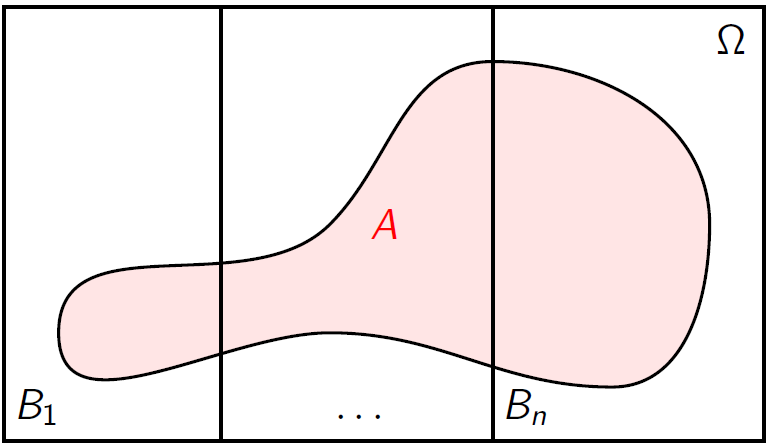
\includegraphics[width=\columnwidth]{images/totale_wahrscheinlichkeit.png}
\end{minipage}
\hfill
\begin{minipage}{0.56\columnwidth}
	\begin{tabular}{r c l }
		$P(Z \cap A)$ 	 	& $=$ 	& $P(Z|A) \cdot P(A)$ \\
		$ + P(Z \cap B)$ 	& $=$ 	& $P(Z|B) \cdot P(B)$ \\
		$ + P(Z \cap C)$ 	& $=$ 	& $P(Z|C) \cdot P(C)$ \\
	\hline
		$P(Z)$ 				& 		& 						\\
	\end{tabular}
\end{minipage}

